\documentclass[11pt]{article}
\usepackage[margin=1in]{geometry}
\usepackage{booktabs}
\usepackage{graphicx}
\usepackage{float}
\usepackage{hyperref}

\title{KinBench-UQ: Methods and Results Draft}
\author{}
\date{}

\begin{document}
\maketitle

\section{Methods}

\subsection{Problem Formulation}

KinBench-UQ studies kinase--ligand candidate prioritization. Given a kinase
target and a set of candidate small molecules, the objective is to estimate
binding strength and rank compounds so that the most promising candidates are
tested first. We frame the task as target-aware affinity prediction with a
primary emphasis on ranking quality under realistic train--test separation.

\subsection{Data and Target Definition}

The primary in-domain dataset is Davis. The repository standardizes assay
measurements into a unified regression target,
\texttt{p\_activity = -log10(affinity in molar units)}, while preserving assay
family metadata in \texttt{affinity\_type}. This avoids silently collapsing
\texttt{K\_d}, \texttt{K\_i}, and \texttt{IC50} into an incorrectly named label.

For external validation, we construct a kinase-focused BindingDB-derived test
set processed into the same schema. The current external panel contains 1,617
rows spanning 8 targets.

\subsection{Benchmark Splits}

We evaluate models on four primary split families used in the current benchmark
results:

\begin{itemize}
  \item \textbf{Random}: standard interaction-level holdout.
  \item \textbf{Cold-target}: evaluation targets are absent from training.
  \item \textbf{Sequence-identity}: target clusters are defined by exact global
  pairwise sequence identity rather than a proxy similarity score.
  \item \textbf{Mutation-holdout}: mutant family members are reserved for
  evaluation while related family context remains in training.
\end{itemize}

The exact sequence-identity split is a central part of the protocol. The saved
leakage summary shows that the mean nearest-train sequence identity falls to
0.367 on this split, compared with 1.000 for several easier Davis split
families, making it a substantially stricter test of target generalization.

\subsection{Compared Models}

We evaluate five models under a common benchmark runner:

\begin{enumerate}
  \item \texttt{ligand\_only\_ridge}
  \item \texttt{ridge\_ensemble}
  \item \texttt{dual\_tower\_uq}
  \item \texttt{deepdta\_exact}
  \item \texttt{graphdta\_gcn\_exact}
\end{enumerate}

The first three are repository baselines. The last two are literature-style
reproductions run under the same split protocol and artifact format as the
repo-native models. The \texttt{dual\_tower\_uq} model is the main target-aware
repository model and additionally produces predictive uncertainty estimates.

\subsection{Evaluation Metrics}

We report:

\begin{itemize}
  \item RMSE
  \item global Spearman correlation
  \item mean per-target Spearman
  \item ROC-AUC at \texttt{p\_activity >= 6.0}
  \item mean top-10\% enrichment
\end{itemize}

For uncertainty-capable models we also report calibrated interval coverage and
prediction spread. In addition to split-level summaries, we export mutation
family analyses and leakage summaries from generated CSV artifacts.

\subsection{Reproducibility}

All result tables and figures are generated from versioned result files in the
repository. The main benchmark summaries are stored in
\texttt{results/benchmark/summary.csv} and
\texttt{results/benchmark/summary.json}. The paper-facing summary is generated
by \texttt{scripts/generate\_paper\_assets.py} and written to
\texttt{paper/generated\_results.md}, with associated plots saved under
\texttt{figures/}.

\section{Results}

\subsection{Overall Benchmark Ranking}

Table~\ref{tab:main-results} summarizes the current four-split benchmark. The
results show that no single model is best on every setting, which is a useful
property of the benchmark. \texttt{deepdta\_exact} is strongest on the easier
\texttt{random} split and also attains the best RMSE on the stricter
\texttt{sequence\_identity} split. In contrast, \texttt{dual\_tower\_uq} is
best on \texttt{cold\_target} and substantially best on
\texttt{mutation\_holdout}, while also retaining the best Spearman correlation
on \texttt{cold\_target}, \texttt{sequence\_identity}, and
\texttt{mutation\_holdout}.

\begin{table}[H]
\centering
\caption{Main benchmark results across the four primary split families. Lower
RMSE is better. Higher Spearman is better.}
\label{tab:main-results}
\begin{tabular}{llcc}
\toprule
Split & Model & RMSE & Spearman \\
\midrule
Random & deepdta\_exact & 0.548 & 0.658 \\
Random & dual\_tower\_uq & 0.596 & 0.634 \\
Random & graphdta\_gcn\_exact & 0.591 & 0.610 \\
\midrule
Cold-target & dual\_tower\_uq & 0.597 & 0.587 \\
Cold-target & deepdta\_exact & 0.614 & 0.563 \\
Cold-target & graphdta\_gcn\_exact & 0.690 & 0.478 \\
\midrule
Sequence-identity & deepdta\_exact & 0.681 & 0.446 \\
Sequence-identity & dual\_tower\_uq & 0.701 & 0.461 \\
Sequence-identity & graphdta\_gcn\_exact & 0.780 & 0.385 \\
\midrule
Mutation-holdout & dual\_tower\_uq & 0.545 & 0.818 \\
Mutation-holdout & graphdta\_gcn\_exact & 0.736 & 0.749 \\
Mutation-holdout & deepdta\_exact & 0.764 & 0.739 \\
\bottomrule
\end{tabular}
\end{table}

These findings sharpen the benchmark narrative. If the paper emphasized only
the easier random split, \texttt{deepdta\_exact} would appear clearly dominant.
However, the more realistic splits reveal a more differentiated picture:
\texttt{dual\_tower\_uq} is better at generalization to unseen targets and
mutation-family transfer, while \texttt{deepdta\_exact} remains very strong on
more standard affinity settings.

\subsection{Sequence-Identity Leakage}

The exact sequence-identity analysis confirms that split choice materially
changes what the benchmark measures. The saved leakage summary shows a mean
nearest-train sequence identity of 0.367 and a maximum of 0.581 for the
\texttt{sequence\_identity} split, whereas several easier split families admit
exact target neighbors. This supports the claim that the stricter split is a
more credible test of biological generalization than standard random
interaction holdout.

\subsection{Mutation-Family Behavior}

The mutation-family analysis reveals that performance is not uniform across
families. \texttt{dual\_tower\_uq} is particularly strong on several mutation
families, including PIK3CA (RMSE 0.150), LRRK2 (0.334), BRAF (0.389), MET
(0.411), and FLT3 (0.520). By contrast, both literature baselines degrade more
substantially on several of these families. This is important because mutation
transfer is a more realistic use case than aggregate in-domain regression
alone.

\subsection{External Validation}

External validation remains substantially harder than in-domain Davis testing.
Among the currently generated external runs, \texttt{dual\_tower\_uq} attains
RMSE 1.484 and mean per-target Spearman 0.342 on the BindingDB-derived
evaluation set, compared with RMSE 1.602 and 1.641 for the target-aware ridge
ensemble and ligand-only ridge baselines, respectively. These numbers are worse
than the in-domain Davis results, but they are more scientifically credible for
a candidate-prioritization claim.

At present, the external validation summary includes the repository baselines
only. Extending the external protocol to the literature baselines would further
strengthen the paper, but the core benchmark comparison on the four primary
splits is already complete.

\subsection{Interpretation}

The current benchmark no longer supports an overly simple ``our model wins
everything'' story, and that is a strength rather than a weakness. The more
defensible conclusion is:

\begin{quote}
KinBench-UQ provides a stricter and more reproducible kinase
candidate-prioritization benchmark, and the repository's
\texttt{dual\_tower\_uq} model remains especially strong on several of the
harder evaluation settings, even in the presence of competitive
literature-style baselines.
\end{quote}

\begin{figure}[H]
\centering
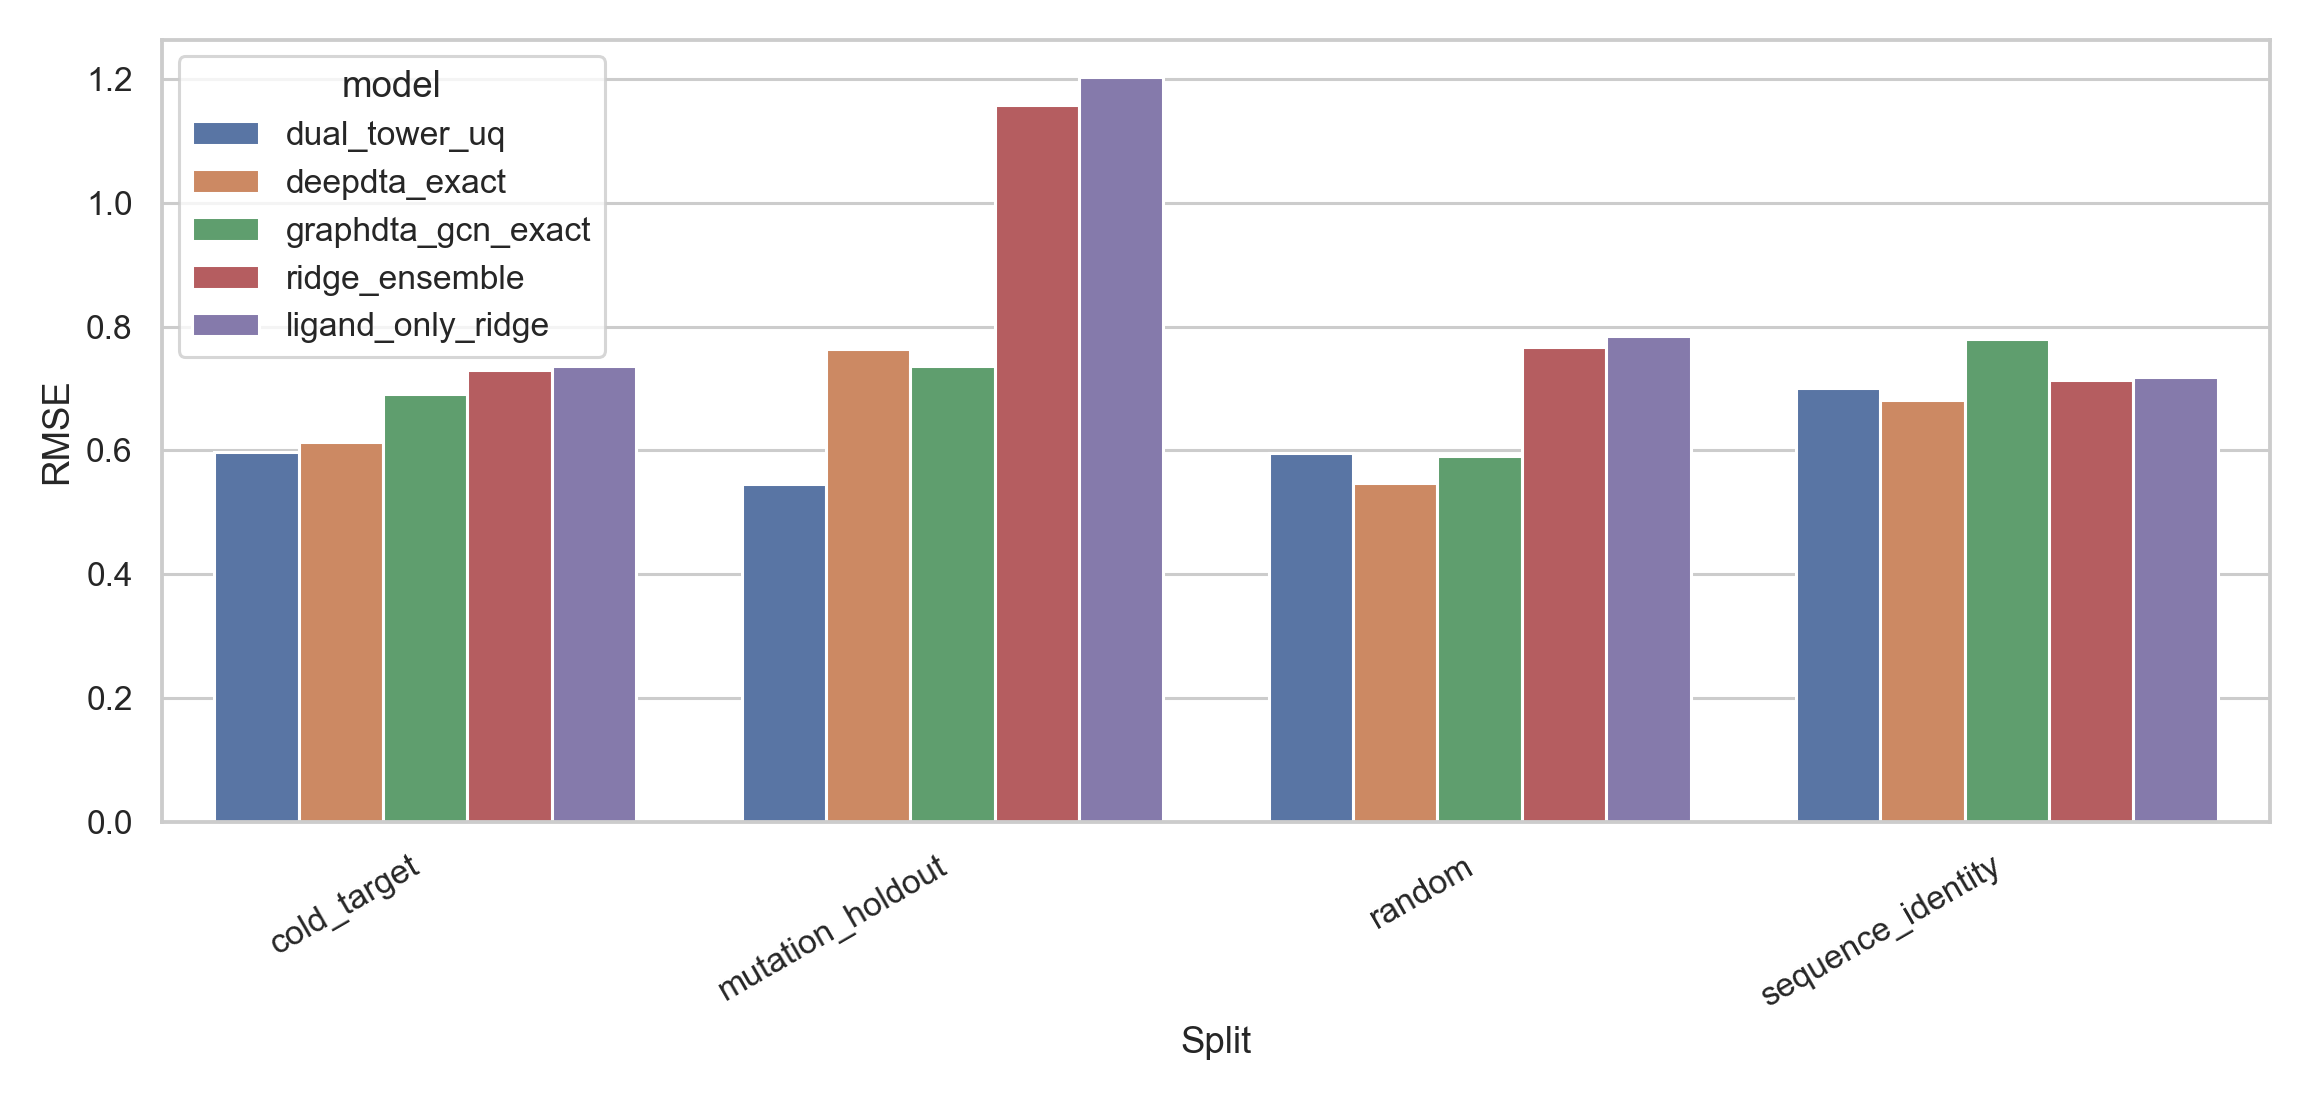
\includegraphics[width=0.85\linewidth]{../figures/split_rmse_comparison.png}
\caption{RMSE comparison across split families.}
\label{fig:rmse}
\end{figure}

\begin{figure}[H]
\centering
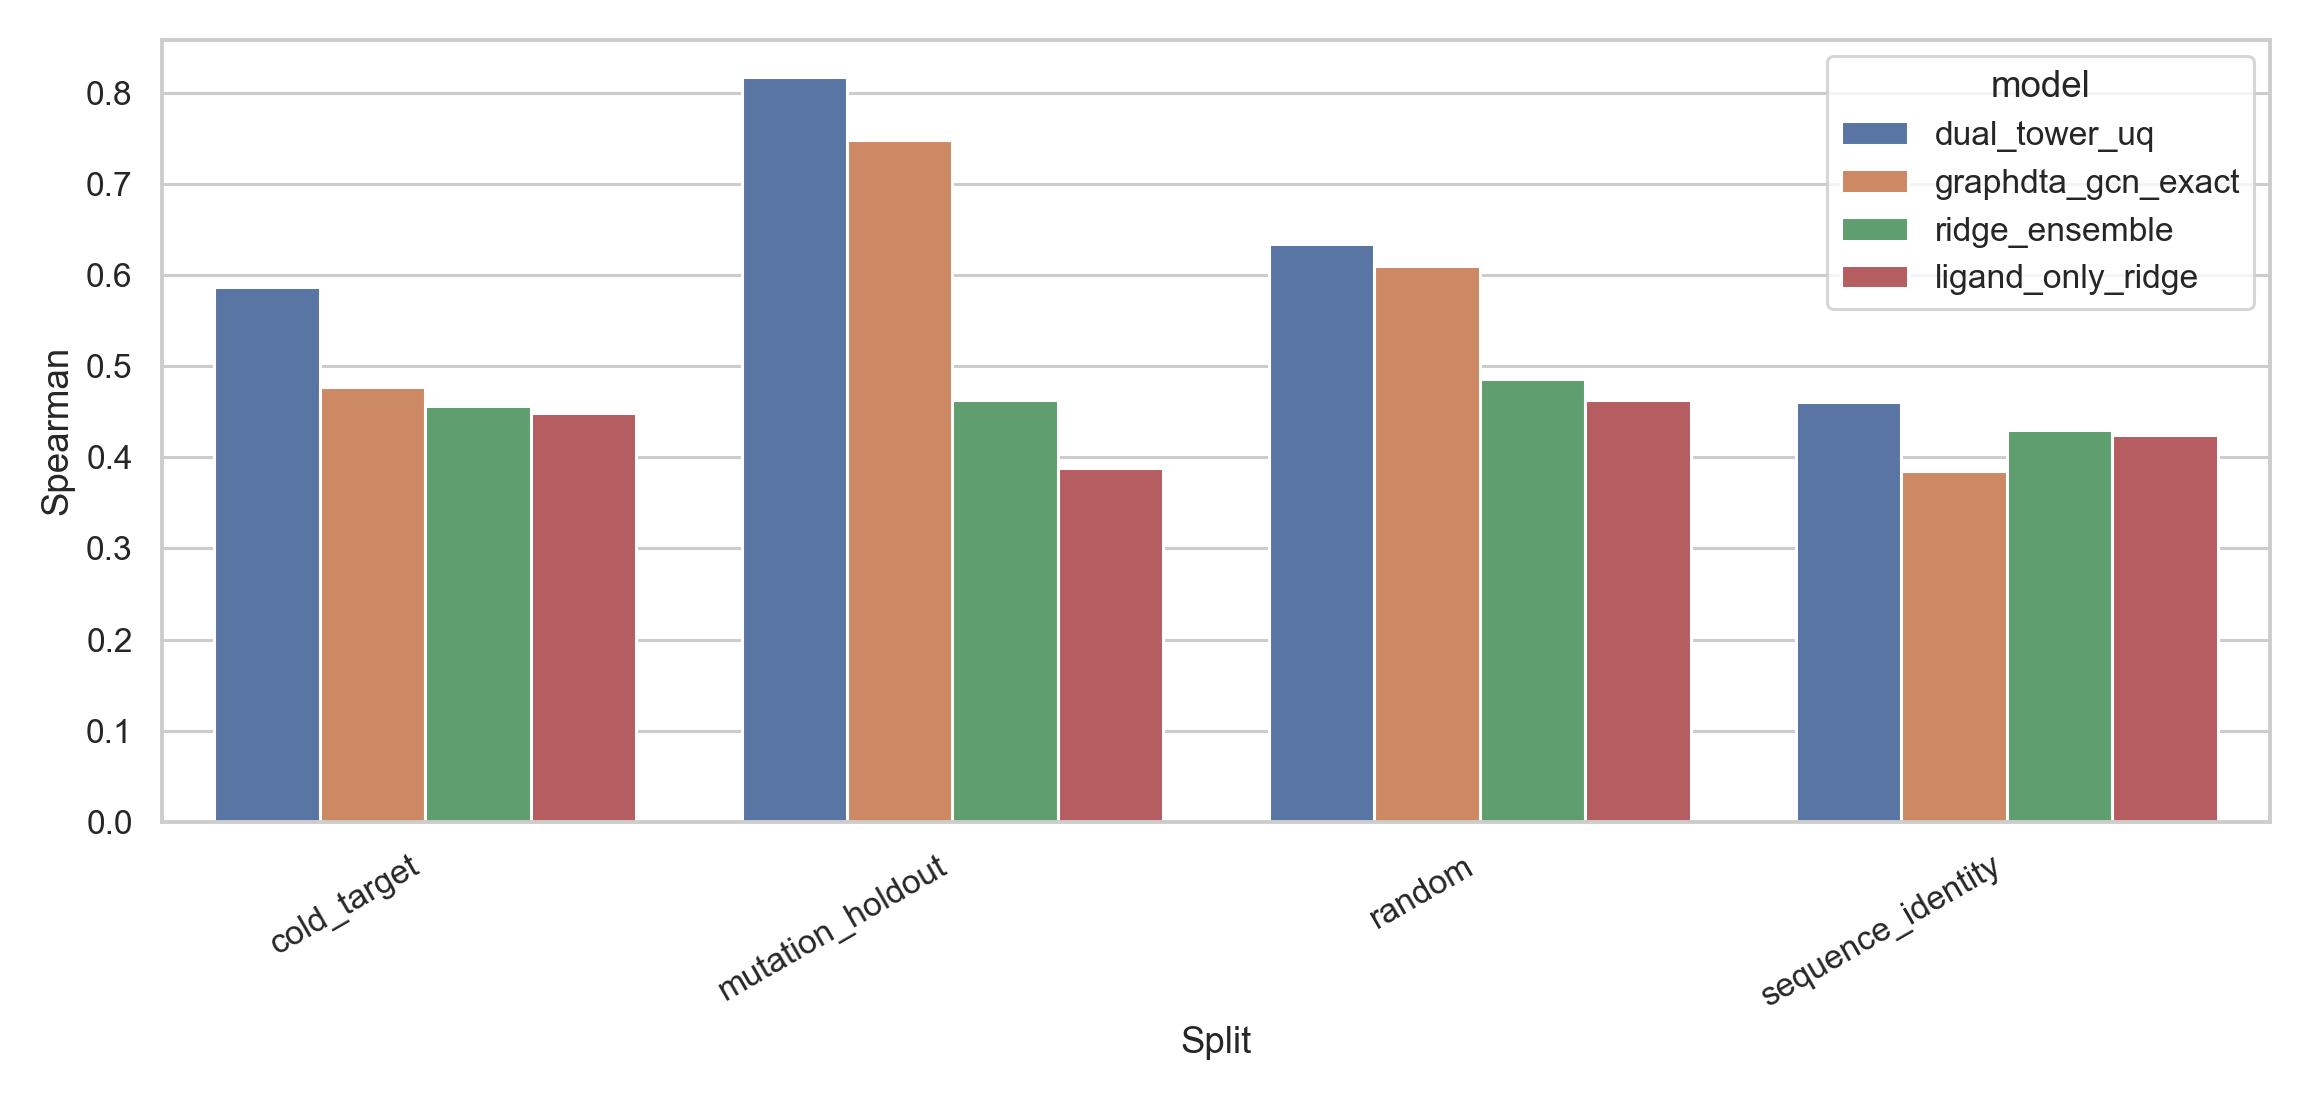
\includegraphics[width=0.85\linewidth]{../figures/split_spearman_comparison.png}
\caption{Spearman comparison across split families.}
\label{fig:spearman}
\end{figure}

\end{document}
